\chapter{Work sharing}

\section{Unmodified program}

\begin{figure}[!h]
  \begin{center}
         \resizebox{160mm}{!}{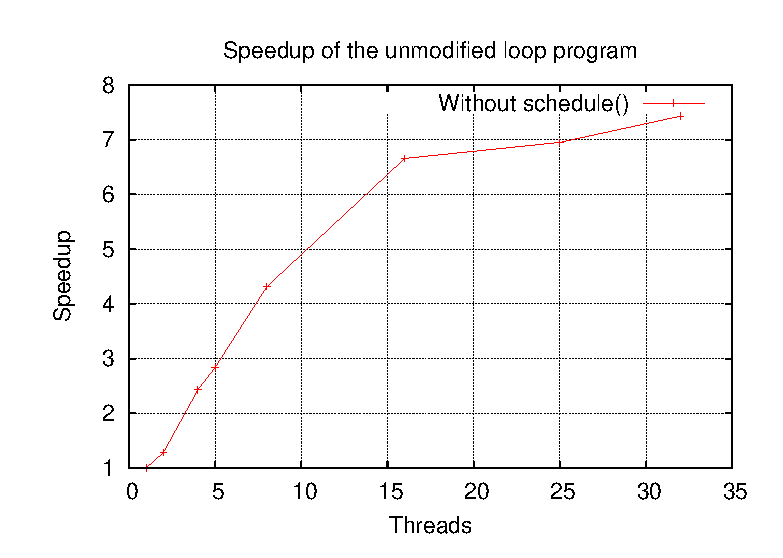
\includegraphics{pic/graph_q4.eps}}
  \end{center}
  \caption{Speedup of the unmodified program}
  \label{unmodif}
\end{figure}

The speedup keeps increasing slowly but is too low for a few threads to jusitfy their use.

\section{Using scheduling directives}

In the graphs \ref{2000} and \ref{10000}, we tried the three directives with an arbitrary sized chunk. The graph \ref{opt} shows the result if we let OpenMP take care of the chunk's size.

\begin{figure}[!h]
  \begin{center}
         \resizebox{160mm}{!}{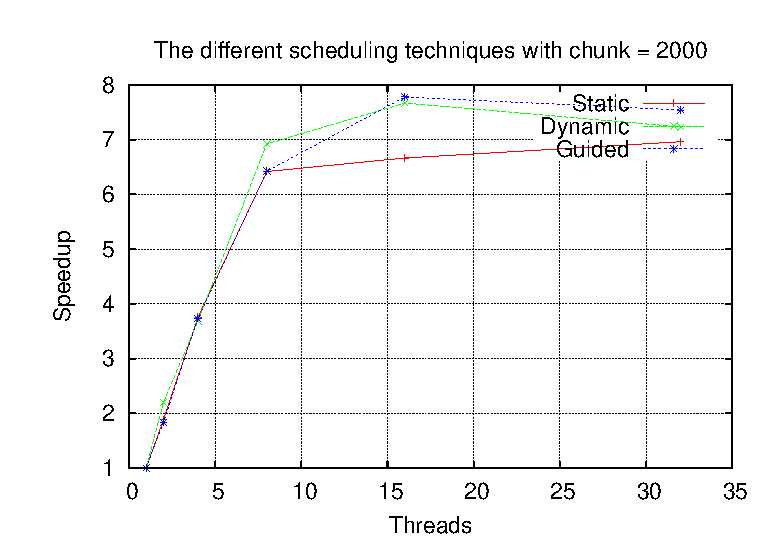
\includegraphics{pic/graph_q4_2000.eps}}
  \end{center}
  \caption{With chunk = 2000}
  \label{2000}
\end{figure}

\begin{figure}[!h]
  \begin{center}
         \resizebox{160mm}{!}{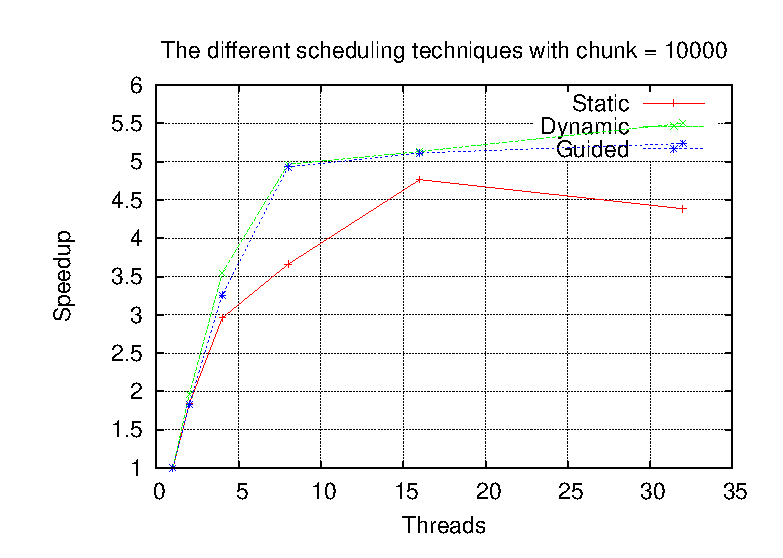
\includegraphics{pic/graph_q4_10000.eps}}
  \end{center}
  \caption{With chunk = 10000}
  \label{10000}
\end{figure}

\begin{figure}[!h]
  \begin{center}
         \resizebox{160mm}{!}{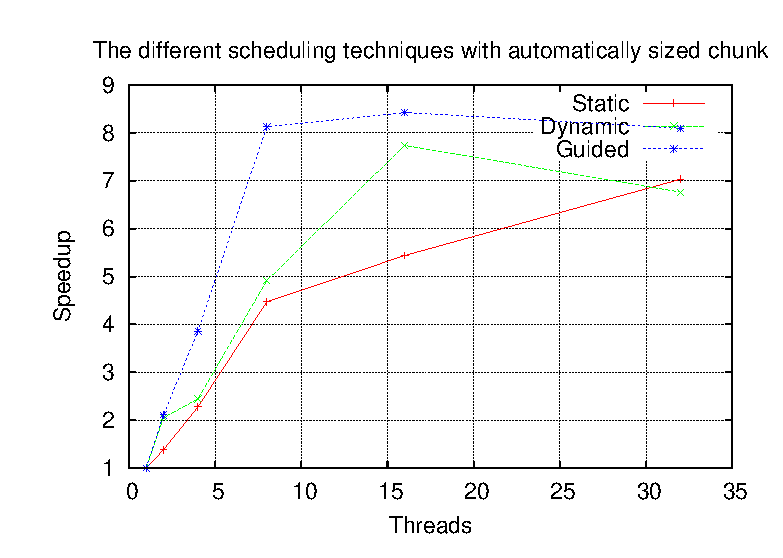
\includegraphics{pic/graph_q4_opt.eps}}
  \end{center}
  \caption{With automatically sized chunk}
  \label{opt}
\end{figure}


The chunk size is important. If is is too big, it will create load imbalance and lead to bad results, as the picture \ref{10000} shows. Too small chunks are not good either as they multiply the number of context switches. 

As we can see, especially with automatically sized chunks,  choosing dynamic or guided scheduling gives the bests results. It is so because the problem was a poor load balance and it is known that both dynamic and guided scheduling are good to avoid this problem. Both dynamic and guided scheduling have very good results with a few number of threads, very close to the optimal speedup (which is simply the number of processors involved). This is not the case of the static scheduling. However, the results start to stagnate passed the 10 threads involved. This is caused by the fact that our problem size does not scale but the overhead keeps increasing.

